\documentclass[twoside]{book}

% Packages required by doxygen
\usepackage{fixltx2e}
\usepackage{calc}
\usepackage{doxygen}
\usepackage[export]{adjustbox} % also loads graphicx
\usepackage{graphicx}
\usepackage[utf8]{inputenc}
\usepackage{makeidx}
\usepackage{multicol}
\usepackage{multirow}
\PassOptionsToPackage{warn}{textcomp}
\usepackage{textcomp}
\usepackage[nointegrals]{wasysym}
\usepackage[table]{xcolor}

% NLS support packages
\usepackage[brazil]{babel}
% Font selection
\usepackage[T1]{fontenc}
\usepackage[scaled=.90]{helvet}
\usepackage{courier}
\usepackage{amssymb}
\usepackage{sectsty}
\renewcommand{\familydefault}{\sfdefault}
\allsectionsfont{%
  \fontseries{bc}\selectfont%
  \color{darkgray}%
}
\renewcommand{\DoxyLabelFont}{%
  \fontseries{bc}\selectfont%
  \color{darkgray}%
}
\newcommand{\+}{\discretionary{\mbox{\scriptsize$\hookleftarrow$}}{}{}}

% Page & text layout
\usepackage{geometry}
\geometry{%
  a4paper,%
  top=2.5cm,%
  bottom=2.5cm,%
  left=2.5cm,%
  right=2.5cm%
}
\tolerance=750
\hfuzz=15pt
\hbadness=750
\setlength{\emergencystretch}{15pt}
\setlength{\parindent}{0cm}
\setlength{\parskip}{3ex plus 2ex minus 2ex}
\makeatletter
\renewcommand{\paragraph}{%
  \@startsection{paragraph}{4}{0ex}{-1.0ex}{1.0ex}{%
    \normalfont\normalsize\bfseries\SS@parafont%
  }%
}
\renewcommand{\subparagraph}{%
  \@startsection{subparagraph}{5}{0ex}{-1.0ex}{1.0ex}{%
    \normalfont\normalsize\bfseries\SS@subparafont%
  }%
}
\makeatother

% Headers & footers
\usepackage{fancyhdr}
\pagestyle{fancyplain}
\fancyhead[LE]{\fancyplain{}{\bfseries\thepage}}
\fancyhead[CE]{\fancyplain{}{}}
\fancyhead[RE]{\fancyplain{}{\bfseries\leftmark}}
\fancyhead[LO]{\fancyplain{}{\bfseries\rightmark}}
\fancyhead[CO]{\fancyplain{}{}}
\fancyhead[RO]{\fancyplain{}{\bfseries\thepage}}
\fancyfoot[LE]{\fancyplain{}{}}
\fancyfoot[CE]{\fancyplain{}{}}
\fancyfoot[RE]{\fancyplain{}{\bfseries\scriptsize Gerado por Doxygen }}
\fancyfoot[LO]{\fancyplain{}{\bfseries\scriptsize Gerado por Doxygen }}
\fancyfoot[CO]{\fancyplain{}{}}
\fancyfoot[RO]{\fancyplain{}{}}
\renewcommand{\footrulewidth}{0.4pt}
\renewcommand{\chaptermark}[1]{%
  \markboth{#1}{}%
}
\renewcommand{\sectionmark}[1]{%
  \markright{\thesection\ #1}%
}

% Indices & bibliography
\usepackage{natbib}
\usepackage[titles]{tocloft}
\setcounter{tocdepth}{3}
\setcounter{secnumdepth}{5}
\makeindex

% Hyperlinks (required, but should be loaded last)
\usepackage{ifpdf}
\ifpdf
  \usepackage[pdftex,pagebackref=true]{hyperref}
\else
  \usepackage[ps2pdf,pagebackref=true]{hyperref}
\fi
\hypersetup{%
  colorlinks=true,%
  linkcolor=blue,%
  citecolor=blue,%
  unicode%
}

% Custom commands
\newcommand{\clearemptydoublepage}{%
  \newpage{\pagestyle{empty}\cleardoublepage}%
}

\usepackage{caption}
\captionsetup{labelsep=space,justification=centering,font={bf},singlelinecheck=off,skip=4pt,position=top}

%===== C O N T E N T S =====

\begin{document}

% Titlepage & ToC
\hypersetup{pageanchor=false,
             bookmarksnumbered=true,
             pdfencoding=unicode
            }
\pagenumbering{alph}
\begin{titlepage}
\vspace*{7cm}
\begin{center}%
{\Large Tratamento de Classes Abstratas \\[1ex]\large 1.\+0 }\\
\vspace*{1cm}
{\large Gerado por Doxygen 1.8.14}\\
\end{center}
\end{titlepage}
\clearemptydoublepage
\pagenumbering{roman}
\tableofcontents
\clearemptydoublepage
\pagenumbering{arabic}
\hypersetup{pageanchor=true}

%--- Begin generated contents ---
\chapter{Índice Hierárquico}
\section{Hierarquia de Classes}
Esta lista de hierarquias está parcialmente ordenada (ordem alfabética)\+:\begin{DoxyCompactList}
\item \contentsline{section}{Figura\+Geometrica}{\pageref{class_figura_geometrica}}{}
\begin{DoxyCompactList}
\item \contentsline{section}{Brush}{\pageref{class_brush}}{}
\item \contentsline{section}{Circulo}{\pageref{class_circulo}}{}
\item \contentsline{section}{Reta}{\pageref{class_reta}}{}
\item \contentsline{section}{Retangulo}{\pageref{class_retangulo}}{}
\end{DoxyCompactList}
\item \contentsline{section}{Screen}{\pageref{class_screen}}{}
\end{DoxyCompactList}

\chapter{Índice dos Componentes}
\section{Lista de Classes}
Aqui estão as classes, estruturas, uniões e interfaces e suas respectivas descrições\+:\begin{DoxyCompactList}
\item\contentsline{section}{\mbox{\hyperlink{class_brush}{Brush}} \\*A classe \mbox{\hyperlink{class_brush}{Brush}} é responsável por caracterizar o brush que será utilizado para o desenho }{\pageref{class_brush}}{}
\item\contentsline{section}{\mbox{\hyperlink{class_circulo}{Circulo}} \\*A classe \mbox{\hyperlink{class_circulo}{Circulo}} é utilizada para representar os círculos que poderão ser desenhados na tela }{\pageref{class_circulo}}{}
\item\contentsline{section}{\mbox{\hyperlink{class_figura_geometrica}{Figura\+Geometrica}} \\*A classe \mbox{\hyperlink{class_figura_geometrica}{Figura\+Geometrica}} é utilizada para representar as figuras que serão desenhadas }{\pageref{class_figura_geometrica}}{}
\item\contentsline{section}{\mbox{\hyperlink{class_reta}{Reta}} \\*A classe \mbox{\hyperlink{class_reta}{Reta}} é utilizada para representar as retas que poderão ser desenhadas na tela }{\pageref{class_reta}}{}
\item\contentsline{section}{\mbox{\hyperlink{class_retangulo}{Retangulo}} \\*A classe \mbox{\hyperlink{class_retangulo}{Retangulo}} é utilizada para representar os retângulos que poderão ser desenhados na tela }{\pageref{class_retangulo}}{}
\item\contentsline{section}{\mbox{\hyperlink{class_screen}{Screen}} \\*A classe \mbox{\hyperlink{class_screen}{Screen}} é utilizada para representar a tela de desenho }{\pageref{class_screen}}{}
\end{DoxyCompactList}

\chapter{Índice dos Arquivos}
\section{Lista de Arquivos}
Esta é a lista de todos os arquivos e suas respectivas descrições\+:\begin{DoxyCompactList}
\item\contentsline{section}{Projeto2\+\_\+\+Tratamentode\+Classes\+Abstratas/\mbox{\hyperlink{brush_8cpp}{brush.\+cpp}} }{\pageref{brush_8cpp}}{}
\item\contentsline{section}{Projeto2\+\_\+\+Tratamentode\+Classes\+Abstratas/\mbox{\hyperlink{brush_8h}{brush.\+h}} }{\pageref{brush_8h}}{}
\item\contentsline{section}{Projeto2\+\_\+\+Tratamentode\+Classes\+Abstratas/\mbox{\hyperlink{circulo_8cpp}{circulo.\+cpp}} }{\pageref{circulo_8cpp}}{}
\item\contentsline{section}{Projeto2\+\_\+\+Tratamentode\+Classes\+Abstratas/\mbox{\hyperlink{circulo_8h}{circulo.\+h}} }{\pageref{circulo_8h}}{}
\item\contentsline{section}{Projeto2\+\_\+\+Tratamentode\+Classes\+Abstratas/\mbox{\hyperlink{figurageometrica_8cpp}{figurageometrica.\+cpp}} }{\pageref{figurageometrica_8cpp}}{}
\item\contentsline{section}{Projeto2\+\_\+\+Tratamentode\+Classes\+Abstratas/\mbox{\hyperlink{figurageometrica_8h}{figurageometrica.\+h}} }{\pageref{figurageometrica_8h}}{}
\item\contentsline{section}{Projeto2\+\_\+\+Tratamentode\+Classes\+Abstratas/\mbox{\hyperlink{main_8cpp}{main.\+cpp}} }{\pageref{main_8cpp}}{}
\item\contentsline{section}{Projeto2\+\_\+\+Tratamentode\+Classes\+Abstratas/\mbox{\hyperlink{reta_8cpp}{reta.\+cpp}} }{\pageref{reta_8cpp}}{}
\item\contentsline{section}{Projeto2\+\_\+\+Tratamentode\+Classes\+Abstratas/\mbox{\hyperlink{reta_8h}{reta.\+h}} }{\pageref{reta_8h}}{}
\item\contentsline{section}{Projeto2\+\_\+\+Tratamentode\+Classes\+Abstratas/\mbox{\hyperlink{retangulo_8cpp}{retangulo.\+cpp}} }{\pageref{retangulo_8cpp}}{}
\item\contentsline{section}{Projeto2\+\_\+\+Tratamentode\+Classes\+Abstratas/\mbox{\hyperlink{retangulo_8h}{retangulo.\+h}} }{\pageref{retangulo_8h}}{}
\item\contentsline{section}{Projeto2\+\_\+\+Tratamentode\+Classes\+Abstratas/\mbox{\hyperlink{screen_8cpp}{screen.\+cpp}} }{\pageref{screen_8cpp}}{}
\item\contentsline{section}{Projeto2\+\_\+\+Tratamentode\+Classes\+Abstratas/\mbox{\hyperlink{screen_8h}{screen.\+h}} }{\pageref{screen_8h}}{}
\end{DoxyCompactList}

\chapter{Classes}
\hypertarget{class_brush}{}\section{Referência da Classe Brush}
\label{class_brush}\index{Brush@{Brush}}


A classe \mbox{\hyperlink{class_brush}{Brush}} é responsável por caracterizar o brush que será utilizado para o desenho.  




{\ttfamily \#include $<$brush.\+h$>$}

Diagrama de hierarquia para Brush\+:\begin{figure}[H]
\begin{center}
\leavevmode
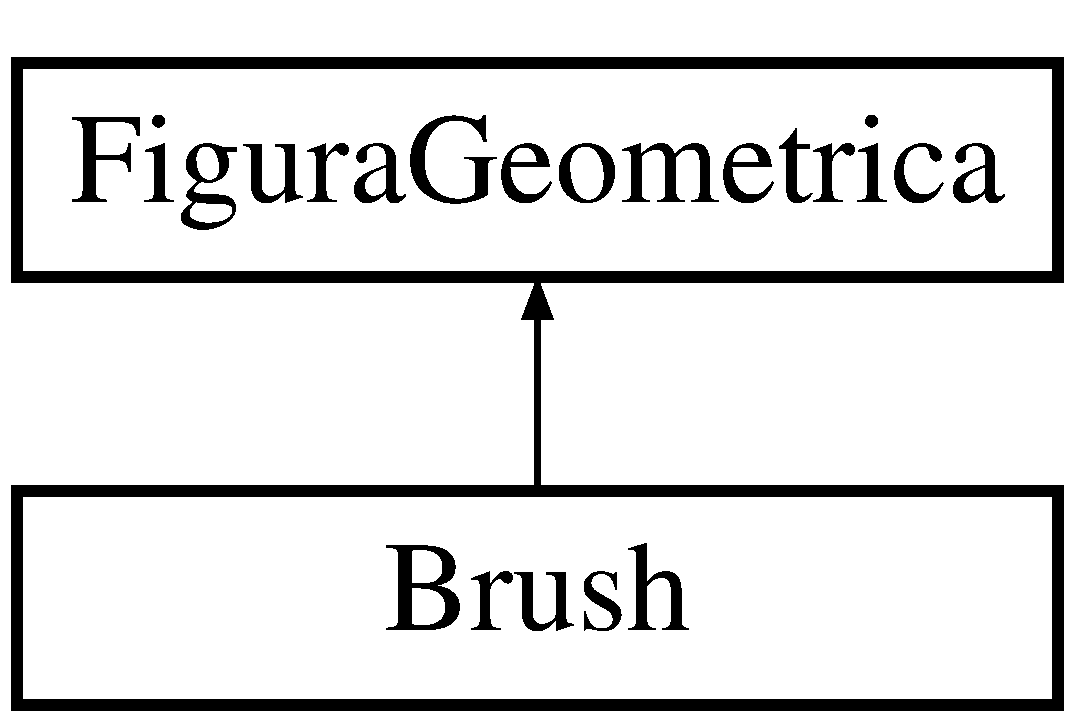
\includegraphics[height=2.000000cm]{class_brush}
\end{center}
\end{figure}
\subsection*{Membros Públicos}
\begin{DoxyCompactItemize}
\item 
\mbox{\hyperlink{class_brush_a5ded381f29fa4566fbce96f623baecab}{Brush}} (char \+\_\+br=\textquotesingle{} \textquotesingle{})
\begin{DoxyCompactList}\small\item\em Construtor \mbox{\hyperlink{class_brush}{Brush}}. \end{DoxyCompactList}\item 
void \mbox{\hyperlink{class_brush_ad12c371aba8d8770df593ef94ae14dd0}{draw}} (\mbox{\hyperlink{class_screen}{Screen}} \&t)
\begin{DoxyCompactList}\small\item\em Método para desenhar figuras com o brush escolhido pelo usuário. \end{DoxyCompactList}\end{DoxyCompactItemize}


\subsection{Descrição detalhada}
A classe \mbox{\hyperlink{class_brush}{Brush}} é responsável por caracterizar o brush que será utilizado para o desenho. 

\subsection{Construtores e Destrutores}
\mbox{\Hypertarget{class_brush_a5ded381f29fa4566fbce96f623baecab}\label{class_brush_a5ded381f29fa4566fbce96f623baecab}} 
\index{Brush@{Brush}!Brush@{Brush}}
\index{Brush@{Brush}!Brush@{Brush}}
\subsubsection{\texorpdfstring{Brush()}{Brush()}}
{\footnotesize\ttfamily Brush\+::\+Brush (\begin{DoxyParamCaption}\item[{char}]{\+\_\+br = {\ttfamily \textquotesingle{}~\textquotesingle{}} }\end{DoxyParamCaption})}



Construtor \mbox{\hyperlink{class_brush}{Brush}}. 


\begin{DoxyCode}
7                     \{
8     br = \_br;
9 \}
\end{DoxyCode}


\subsection{Funções membros}
\mbox{\Hypertarget{class_brush_ad12c371aba8d8770df593ef94ae14dd0}\label{class_brush_ad12c371aba8d8770df593ef94ae14dd0}} 
\index{Brush@{Brush}!draw@{draw}}
\index{draw@{draw}!Brush@{Brush}}
\subsubsection{\texorpdfstring{draw()}{draw()}}
{\footnotesize\ttfamily void Brush\+::draw (\begin{DoxyParamCaption}\item[{\mbox{\hyperlink{class_screen}{Screen}} \&}]{t }\end{DoxyParamCaption})\hspace{0.3cm}{\ttfamily [virtual]}}



Método para desenhar figuras com o brush escolhido pelo usuário. 



Implementa \mbox{\hyperlink{class_figura_geometrica_a8ee8dedc060b6059a805ea091aef2c41}{Figura\+Geometrica}}.


\begin{DoxyCode}
11                          \{
12     t.\mbox{\hyperlink{class_screen_aebc4eb6cb5acf15a0f04c1494622ab23}{setBrush}}(br);
13 \}
\end{DoxyCode}


A documentação para essa classe foi gerada a partir dos seguintes arquivos\+:\begin{DoxyCompactItemize}
\item 
Projeto2\+\_\+\+Tratamentode\+Classes\+Abstratas/\mbox{\hyperlink{brush_8h}{brush.\+h}}\item 
Projeto2\+\_\+\+Tratamentode\+Classes\+Abstratas/\mbox{\hyperlink{brush_8cpp}{brush.\+cpp}}\end{DoxyCompactItemize}

\hypertarget{class_circulo}{}\section{Referência da Classe Circulo}
\label{class_circulo}\index{Circulo@{Circulo}}


A classe \mbox{\hyperlink{class_circulo}{Circulo}} é utilizada para representar os círculos que poderão ser desenhados na tela.  




{\ttfamily \#include $<$circulo.\+h$>$}

Diagrama de hierarquia para Circulo\+:\begin{figure}[H]
\begin{center}
\leavevmode
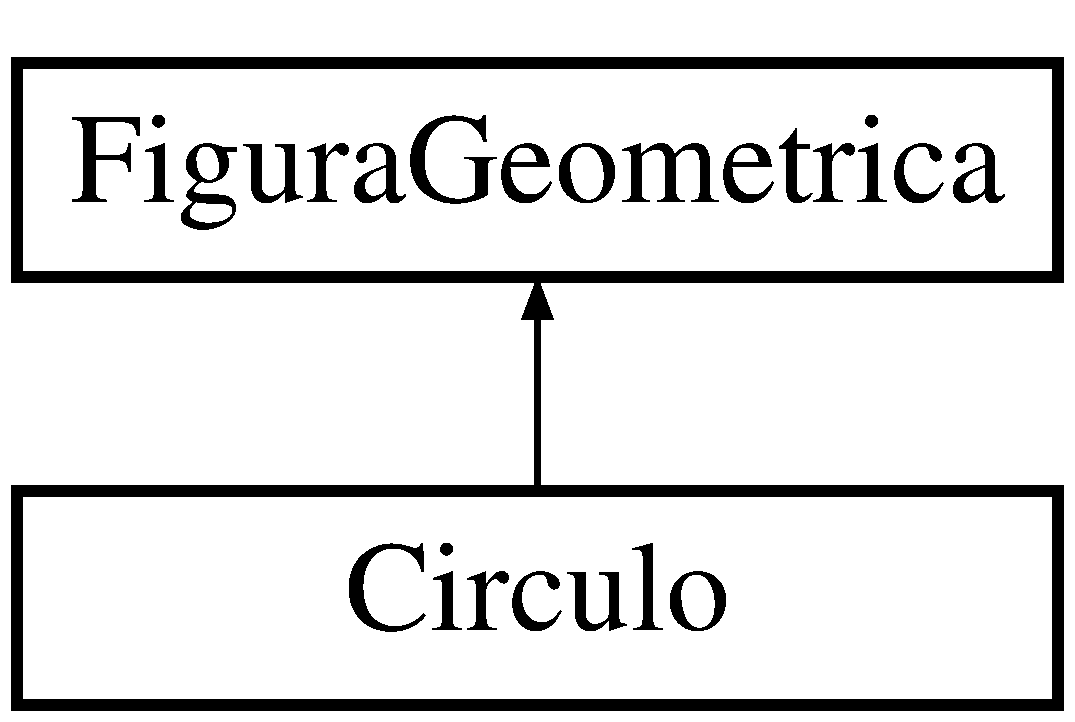
\includegraphics[height=2.000000cm]{class_circulo}
\end{center}
\end{figure}
\subsection*{Membros Públicos}
\begin{DoxyCompactItemize}
\item 
\mbox{\hyperlink{class_circulo_ad460c0782d1a35324cd71079f80e3388}{Circulo}} (int \+\_\+x, int \+\_\+y, int \+\_\+r, bool \+\_\+preenchido)
\begin{DoxyCompactList}\small\item\em Construtor \mbox{\hyperlink{class_circulo}{Circulo}}. \end{DoxyCompactList}\item 
void \mbox{\hyperlink{class_circulo_a593787d6e0618c2eded23e8839e7bea6}{draw}} (\mbox{\hyperlink{class_screen}{Screen}} \&t)
\begin{DoxyCompactList}\small\item\em Método para desenhar o circulo. \end{DoxyCompactList}\item 
void \mbox{\hyperlink{class_circulo_a197439e429d6636a4a43d77e02b20486}{pontos\+Da\+Circunferencia}} (int x1, int y1, \mbox{\hyperlink{class_screen}{Screen}} \&t)
\begin{DoxyCompactList}\small\item\em Método para determinar os pontos da circunferência. \end{DoxyCompactList}\end{DoxyCompactItemize}


\subsection{Descrição detalhada}
A classe \mbox{\hyperlink{class_circulo}{Circulo}} é utilizada para representar os círculos que poderão ser desenhados na tela. 

\subsection{Construtores e Destrutores}
\mbox{\Hypertarget{class_circulo_ad460c0782d1a35324cd71079f80e3388}\label{class_circulo_ad460c0782d1a35324cd71079f80e3388}} 
\index{Circulo@{Circulo}!Circulo@{Circulo}}
\index{Circulo@{Circulo}!Circulo@{Circulo}}
\subsubsection{\texorpdfstring{Circulo()}{Circulo()}}
{\footnotesize\ttfamily Circulo\+::\+Circulo (\begin{DoxyParamCaption}\item[{int}]{\+\_\+x,  }\item[{int}]{\+\_\+y,  }\item[{int}]{\+\_\+r,  }\item[{bool}]{\+\_\+preenchido }\end{DoxyParamCaption})}



Construtor \mbox{\hyperlink{class_circulo}{Circulo}}. 

Um círculo é especificado conforme a posição do centro, seu raio e se este deverá ser preenchido ou apenas o contorno será desenhado 
\begin{DoxyParams}{Parâmetros}
{\em \+\_\+x} & é a posição x do centro do circulo \\
\hline
{\em \+\_\+y} & é a posição y do centro do circulo \\
\hline
{\em \+\_\+r} & é o raio do circulo \\
\hline
{\em \+\_\+preenchido} & determina se o circulo será preenchido ou não \\
\hline
\end{DoxyParams}

\begin{DoxyCode}
9 \{
10     raio = \_r;
11     x = \_x;
12     y = \_y;
13     preenchido = \_preenchido;
14     oct = 1;
15 \}
\end{DoxyCode}


\subsection{Funções membros}
\mbox{\Hypertarget{class_circulo_a593787d6e0618c2eded23e8839e7bea6}\label{class_circulo_a593787d6e0618c2eded23e8839e7bea6}} 
\index{Circulo@{Circulo}!draw@{draw}}
\index{draw@{draw}!Circulo@{Circulo}}
\subsubsection{\texorpdfstring{draw()}{draw()}}
{\footnotesize\ttfamily void Circulo\+::draw (\begin{DoxyParamCaption}\item[{\mbox{\hyperlink{class_screen}{Screen}} \&}]{t }\end{DoxyParamCaption})\hspace{0.3cm}{\ttfamily [virtual]}}



Método para desenhar o circulo. 

Para o desenho do círculo, é verificado se cada coordenada atende à equação do círculo. O algoritmo de Bresenham é utilizado para o desenho do círculo não preenchido. 

Implementa \mbox{\hyperlink{class_figura_geometrica_a8ee8dedc060b6059a805ea091aef2c41}{Figura\+Geometrica}}.


\begin{DoxyCode}
17                            \{
18 
19     \textcolor{keywordflow}{if}(preenchido)\{
20         \textcolor{comment}{//R²= x² + y²}
21 
22         \textcolor{keywordflow}{for}(\textcolor{keywordtype}{int} i=(x-raio);i<=(x+raio);i++)\{
23 
24             \textcolor{keywordflow}{for}(\textcolor{keywordtype}{int} j=(y-raio);j<=(y+raio);j++)\{
25 
26                 \textcolor{keywordflow}{if}( (i-x)*(i-x)+(j-y)*(j-y) <= (raio*raio))\{
27 
28                     t.\mbox{\hyperlink{class_screen_ae6bea81c57a22d226507c3c26fa95ee0}{setPixel}}(i,j);
29                 \}
30             \}
31         \}
32     \}
33 
34     \textcolor{keywordflow}{else}\{
35         \textcolor{keywordtype}{int} x1 = 0;
36         \textcolor{keywordtype}{int} y1 = raio;
37         \textcolor{keywordtype}{int} d = 1 - raio;
38         \mbox{\hyperlink{class_circulo_a197439e429d6636a4a43d77e02b20486}{pontosDaCircunferencia}}(x1,y1,t);
39 
40         \textcolor{keywordflow}{while}(y1 > x1)\{
41             \textcolor{keywordflow}{if}(d < 0)\{
42 
43                 d = d + 2*x1 + 3;
44                 x1 = x1 + 1;
45             \}
46 
47             \textcolor{keywordflow}{else}\{
48 
49                 d = d + 2*(x1-y1) + 5;
50                 x1 = x1 + 1;
51                 y1 = y1 - 1;
52             \}
53 
54             \mbox{\hyperlink{class_circulo_a197439e429d6636a4a43d77e02b20486}{pontosDaCircunferencia}}(x1,y1,t);
55         \}
56     \}
57 
58 \}
\end{DoxyCode}
\mbox{\Hypertarget{class_circulo_a197439e429d6636a4a43d77e02b20486}\label{class_circulo_a197439e429d6636a4a43d77e02b20486}} 
\index{Circulo@{Circulo}!pontos\+Da\+Circunferencia@{pontos\+Da\+Circunferencia}}
\index{pontos\+Da\+Circunferencia@{pontos\+Da\+Circunferencia}!Circulo@{Circulo}}
\subsubsection{\texorpdfstring{pontos\+Da\+Circunferencia()}{pontosDaCircunferencia()}}
{\footnotesize\ttfamily void Circulo\+::pontos\+Da\+Circunferencia (\begin{DoxyParamCaption}\item[{int}]{x1,  }\item[{int}]{y1,  }\item[{\mbox{\hyperlink{class_screen}{Screen}} \&}]{t }\end{DoxyParamCaption})}



Método para determinar os pontos da circunferência. 

Determina os demais pontos da circunferência, a partir dos pontos do primeiro octante. 
\begin{DoxyCode}
60                                                              \{
61     t.\mbox{\hyperlink{class_screen_ae6bea81c57a22d226507c3c26fa95ee0}{setPixel}}(x + x1, y + y1);
62     t.\mbox{\hyperlink{class_screen_ae6bea81c57a22d226507c3c26fa95ee0}{setPixel}}(x + y1, y + x1);
63     t.\mbox{\hyperlink{class_screen_ae6bea81c57a22d226507c3c26fa95ee0}{setPixel}}(x - y1, y + x1);
64     t.\mbox{\hyperlink{class_screen_ae6bea81c57a22d226507c3c26fa95ee0}{setPixel}}(x - x1, y + y1);
65     t.\mbox{\hyperlink{class_screen_ae6bea81c57a22d226507c3c26fa95ee0}{setPixel}}(x - x1, y - y1);
66     t.\mbox{\hyperlink{class_screen_ae6bea81c57a22d226507c3c26fa95ee0}{setPixel}}(x - y1, y - x1);
67     t.\mbox{\hyperlink{class_screen_ae6bea81c57a22d226507c3c26fa95ee0}{setPixel}}(x + y1, y - x1);
68     t.\mbox{\hyperlink{class_screen_ae6bea81c57a22d226507c3c26fa95ee0}{setPixel}}(x + x1, y - y1);
69 \}
\end{DoxyCode}


A documentação para essa classe foi gerada a partir dos seguintes arquivos\+:\begin{DoxyCompactItemize}
\item 
Projeto2\+\_\+\+Tratamentode\+Classes\+Abstratas/\mbox{\hyperlink{circulo_8h}{circulo.\+h}}\item 
Projeto2\+\_\+\+Tratamentode\+Classes\+Abstratas/\mbox{\hyperlink{circulo_8cpp}{circulo.\+cpp}}\end{DoxyCompactItemize}

\hypertarget{class_figura_geometrica}{}\section{Referência da Classe Figura\+Geometrica}
\label{class_figura_geometrica}\index{Figura\+Geometrica@{Figura\+Geometrica}}


A classe \mbox{\hyperlink{class_figura_geometrica}{Figura\+Geometrica}} é utilizada para representar as figuras que serão desenhadas.  




{\ttfamily \#include $<$figurageometrica.\+h$>$}

Diagrama de hierarquia para Figura\+Geometrica\+:\begin{figure}[H]
\begin{center}
\leavevmode
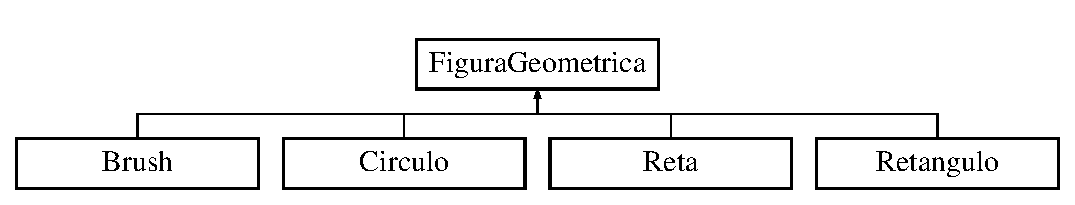
\includegraphics[height=2.000000cm]{class_figura_geometrica}
\end{center}
\end{figure}
\subsection*{Membros Públicos}
\begin{DoxyCompactItemize}
\item 
\mbox{\hyperlink{class_figura_geometrica_a81d7c7efaea511e60a15f5a363138dd9}{Figura\+Geometrica}} ()
\item 
virtual void \mbox{\hyperlink{class_figura_geometrica_a8ee8dedc060b6059a805ea091aef2c41}{draw}} (\mbox{\hyperlink{class_screen}{Screen}} \&t)=0
\begin{DoxyCompactList}\small\item\em Método draw que cria uma tela do tipo \mbox{\hyperlink{class_screen}{Screen}} para permitir o desenho das figuras. \end{DoxyCompactList}\end{DoxyCompactItemize}


\subsection{Descrição detalhada}
A classe \mbox{\hyperlink{class_figura_geometrica}{Figura\+Geometrica}} é utilizada para representar as figuras que serão desenhadas. 

\subsection{Construtores e Destrutores}
\mbox{\Hypertarget{class_figura_geometrica_a81d7c7efaea511e60a15f5a363138dd9}\label{class_figura_geometrica_a81d7c7efaea511e60a15f5a363138dd9}} 
\index{Figura\+Geometrica@{Figura\+Geometrica}!Figura\+Geometrica@{Figura\+Geometrica}}
\index{Figura\+Geometrica@{Figura\+Geometrica}!Figura\+Geometrica@{Figura\+Geometrica}}
\subsubsection{\texorpdfstring{Figura\+Geometrica()}{FiguraGeometrica()}}
{\footnotesize\ttfamily Figura\+Geometrica\+::\+Figura\+Geometrica (\begin{DoxyParamCaption}{ }\end{DoxyParamCaption})}


\begin{DoxyCode}
8 \{
9 
10 \}
\end{DoxyCode}


\subsection{Funções membros}
\mbox{\Hypertarget{class_figura_geometrica_a8ee8dedc060b6059a805ea091aef2c41}\label{class_figura_geometrica_a8ee8dedc060b6059a805ea091aef2c41}} 
\index{Figura\+Geometrica@{Figura\+Geometrica}!draw@{draw}}
\index{draw@{draw}!Figura\+Geometrica@{Figura\+Geometrica}}
\subsubsection{\texorpdfstring{draw()}{draw()}}
{\footnotesize\ttfamily virtual void Figura\+Geometrica\+::draw (\begin{DoxyParamCaption}\item[{\mbox{\hyperlink{class_screen}{Screen}} \&}]{t }\end{DoxyParamCaption})\hspace{0.3cm}{\ttfamily [pure virtual]}}



Método draw que cria uma tela do tipo \mbox{\hyperlink{class_screen}{Screen}} para permitir o desenho das figuras. 


\begin{DoxyParams}{Parâmetros}
{\em t} & é o parâmetro utilizado para receber a tela virtual. \\
\hline
\end{DoxyParams}


Implementado por \mbox{\hyperlink{class_retangulo_ac088dd6d3f4f3d3f80363a868c2e74f1}{Retangulo}}, \mbox{\hyperlink{class_circulo_a593787d6e0618c2eded23e8839e7bea6}{Circulo}}, \mbox{\hyperlink{class_reta_ac2e9805183cd474b62bffd8b032cd780}{Reta}} e \mbox{\hyperlink{class_brush_ad12c371aba8d8770df593ef94ae14dd0}{Brush}}.



A documentação para essa classe foi gerada a partir dos seguintes arquivos\+:\begin{DoxyCompactItemize}
\item 
Projeto2\+\_\+\+Tratamentode\+Classes\+Abstratas/\mbox{\hyperlink{figurageometrica_8h}{figurageometrica.\+h}}\item 
Projeto2\+\_\+\+Tratamentode\+Classes\+Abstratas/\mbox{\hyperlink{figurageometrica_8cpp}{figurageometrica.\+cpp}}\end{DoxyCompactItemize}

\hypertarget{class_reta}{}\section{Referência da Classe Reta}
\label{class_reta}\index{Reta@{Reta}}


A classe \mbox{\hyperlink{class_reta}{Reta}} é utilizada para representar as retas que poderão ser desenhadas na tela.  




{\ttfamily \#include $<$reta.\+h$>$}

Diagrama de hierarquia para Reta\+:\begin{figure}[H]
\begin{center}
\leavevmode
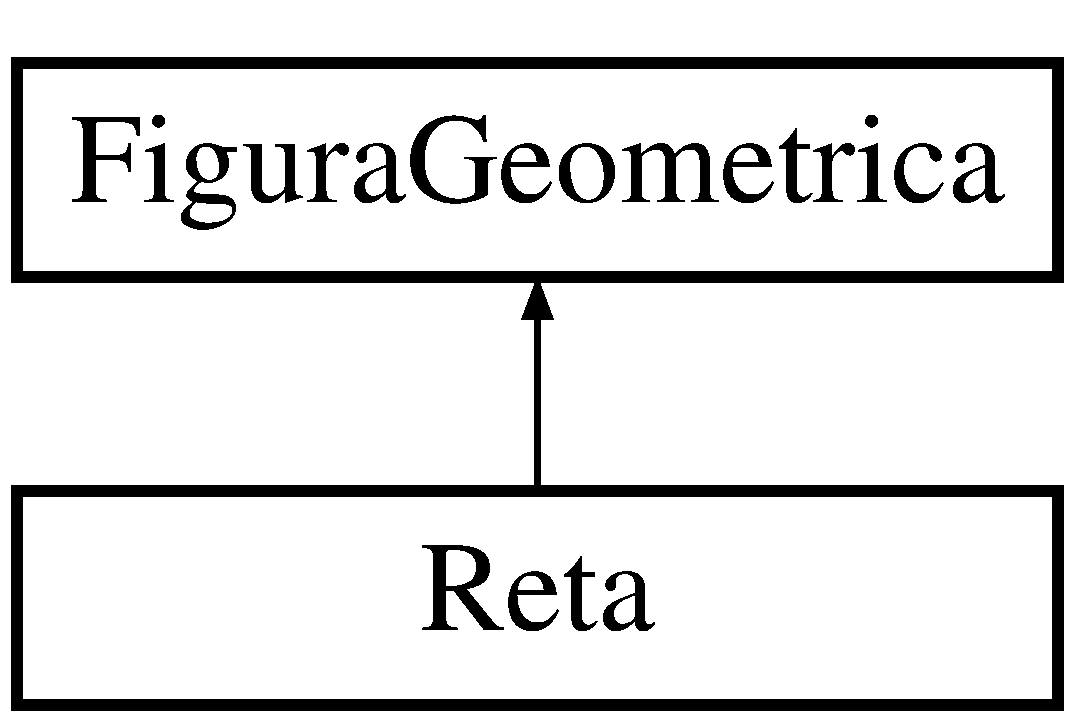
\includegraphics[height=2.000000cm]{class_reta}
\end{center}
\end{figure}
\subsection*{Membros Públicos}
\begin{DoxyCompactItemize}
\item 
\mbox{\hyperlink{class_reta_aa31eee96b0a044711a24907f18f2d2fb}{Reta}} (int \+\_\+xi=0, int \+\_\+yi=0, int \+\_\+xf=0, int \+\_\+yf=0)
\begin{DoxyCompactList}\small\item\em \mbox{\hyperlink{class_reta_aa31eee96b0a044711a24907f18f2d2fb}{Reta\+::\+Reta}}. \end{DoxyCompactList}\item 
void \mbox{\hyperlink{class_reta_ac2e9805183cd474b62bffd8b032cd780}{draw}} (\mbox{\hyperlink{class_screen}{Screen}} \&t)
\begin{DoxyCompactList}\small\item\em Método para desenhar a reta. \end{DoxyCompactList}\end{DoxyCompactItemize}


\subsection{Descrição detalhada}
A classe \mbox{\hyperlink{class_reta}{Reta}} é utilizada para representar as retas que poderão ser desenhadas na tela. 

\subsection{Construtores e Destrutores}
\mbox{\Hypertarget{class_reta_aa31eee96b0a044711a24907f18f2d2fb}\label{class_reta_aa31eee96b0a044711a24907f18f2d2fb}} 
\index{Reta@{Reta}!Reta@{Reta}}
\index{Reta@{Reta}!Reta@{Reta}}
\subsubsection{\texorpdfstring{Reta()}{Reta()}}
{\footnotesize\ttfamily Reta\+::\+Reta (\begin{DoxyParamCaption}\item[{int}]{\+\_\+xi = {\ttfamily 0},  }\item[{int}]{\+\_\+yi = {\ttfamily 0},  }\item[{int}]{\+\_\+xf = {\ttfamily 0},  }\item[{int}]{\+\_\+yf = {\ttfamily 0} }\end{DoxyParamCaption})}



\mbox{\hyperlink{class_reta_aa31eee96b0a044711a24907f18f2d2fb}{Reta\+::\+Reta}}. 

Uma reta é especificada conforme a posição de dois pontos fornecidos. 
\begin{DoxyParams}{Parâmetros}
{\em \+\_\+xi} & coordenada x do ponto inicial da reta \\
\hline
{\em \+\_\+yi} & coordenada y do ponto inicial da reta \\
\hline
{\em \+\_\+xf} & coordenada x do ponto final da reta \\
\hline
{\em \+\_\+yf} & coordenada y do ponto final da reta \\
\hline
\end{DoxyParams}

\begin{DoxyCode}
9                                             \{
10     xi = \_xi; \textcolor{comment}{//alocando nas variáveis privadas}
11     yi = \_yi;
12     xf = \_xf;
13     yf = \_yf;
14 
15 \}
\end{DoxyCode}


\subsection{Funções membros}
\mbox{\Hypertarget{class_reta_ac2e9805183cd474b62bffd8b032cd780}\label{class_reta_ac2e9805183cd474b62bffd8b032cd780}} 
\index{Reta@{Reta}!draw@{draw}}
\index{draw@{draw}!Reta@{Reta}}
\subsubsection{\texorpdfstring{draw()}{draw()}}
{\footnotesize\ttfamily void Reta\+::draw (\begin{DoxyParamCaption}\item[{\mbox{\hyperlink{class_screen}{Screen}} \&}]{t }\end{DoxyParamCaption})\hspace{0.3cm}{\ttfamily [virtual]}}



Método para desenhar a reta. 

O algoritmo de Bresenham é utilizado para aproximar o desenho da reta real. 

Implementa \mbox{\hyperlink{class_figura_geometrica_a8ee8dedc060b6059a805ea091aef2c41}{Figura\+Geometrica}}.


\begin{DoxyCode}
16                         \{
17 
18 \textcolor{keywordtype}{float} Tamanho;
19     \textcolor{keywordtype}{float} Delta\_x;
20     \textcolor{keywordtype}{float} Delta\_y;
21     \textcolor{keywordtype}{float} x = xi;
22     \textcolor{keywordtype}{float} y = yi;
23 
24 
25     \textcolor{keywordflow}{if}( abs(xf-xi) > abs(yf-yi))\{
26         Tamanho = abs(xf-xi);
27     \}
28     \textcolor{keywordflow}{else} \{
29         Tamanho = abs(yf-yi);
30     \}
31 
32     Delta\_x = (xf-xi)/Tamanho;
33     Delta\_y = (yf-yi)/Tamanho;
34     \textcolor{keywordtype}{int} i = 1;
35     \textcolor{keywordflow}{while}(i < Tamanho)\{
36 
37         t.\mbox{\hyperlink{class_screen_ae6bea81c57a22d226507c3c26fa95ee0}{setPixel}}(round(x), round(y));
38         x = x + Delta\_x;
39         y = y + Delta\_y;
40         i++;
41     \}
42 
43 \}
\end{DoxyCode}


A documentação para essa classe foi gerada a partir dos seguintes arquivos\+:\begin{DoxyCompactItemize}
\item 
Projeto2\+\_\+\+Tratamentode\+Classes\+Abstratas/\mbox{\hyperlink{reta_8h}{reta.\+h}}\item 
Projeto2\+\_\+\+Tratamentode\+Classes\+Abstratas/\mbox{\hyperlink{reta_8cpp}{reta.\+cpp}}\end{DoxyCompactItemize}

\hypertarget{class_retangulo}{}\section{Referência da Classe Retangulo}
\label{class_retangulo}\index{Retangulo@{Retangulo}}


A classe \mbox{\hyperlink{class_retangulo}{Retangulo}} é utilizada para representar os retângulos que poderão ser desenhados na tela.  




{\ttfamily \#include $<$retangulo.\+h$>$}

Diagrama de hierarquia para Retangulo\+:\begin{figure}[H]
\begin{center}
\leavevmode
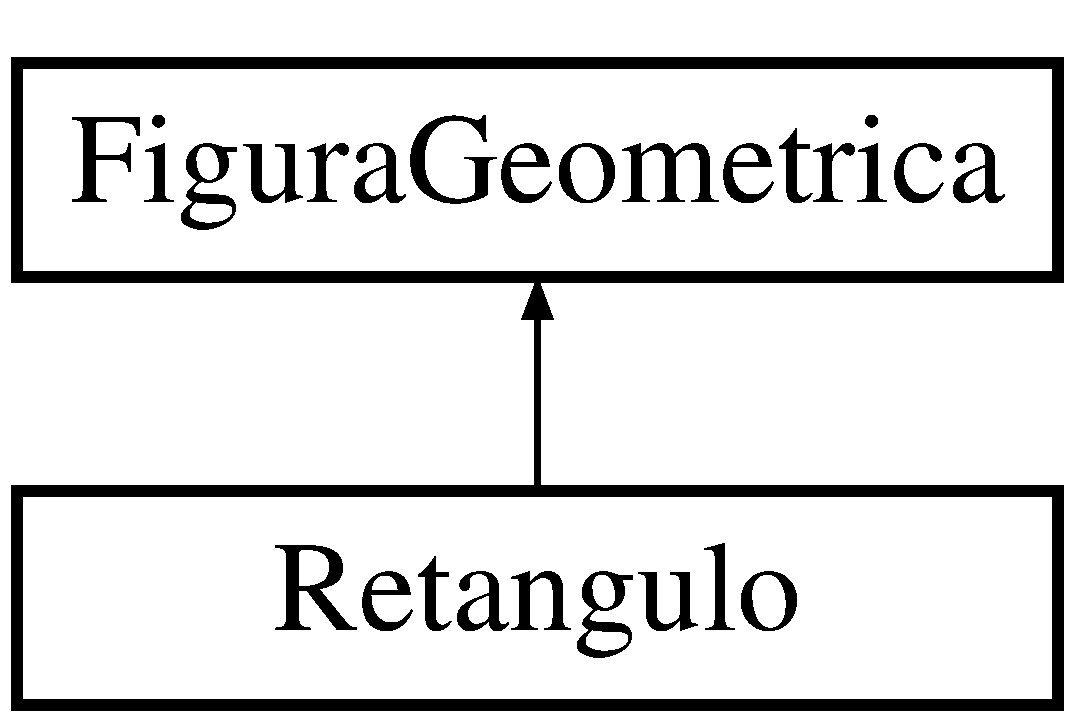
\includegraphics[height=2.000000cm]{class_retangulo}
\end{center}
\end{figure}
\subsection*{Membros Públicos}
\begin{DoxyCompactItemize}
\item 
\mbox{\hyperlink{class_retangulo_a6c53c1dbd4fa3a699f688e29647397c8}{Retangulo}} (int \+\_\+x=0, int \+\_\+y=0, int \+\_\+l=0, int \+\_\+a=0, bool \+\_\+preenchido=false)
\begin{DoxyCompactList}\small\item\em Construtor \mbox{\hyperlink{class_retangulo}{Retangulo}}. \end{DoxyCompactList}\item 
void \mbox{\hyperlink{class_retangulo_ac088dd6d3f4f3d3f80363a868c2e74f1}{draw}} (\mbox{\hyperlink{class_screen}{Screen}} \&t)
\begin{DoxyCompactList}\small\item\em Método para desenhar o retângulo. \end{DoxyCompactList}\end{DoxyCompactItemize}


\subsection{Descrição detalhada}
A classe \mbox{\hyperlink{class_retangulo}{Retangulo}} é utilizada para representar os retângulos que poderão ser desenhados na tela. 

\subsection{Construtores e Destrutores}
\mbox{\Hypertarget{class_retangulo_a6c53c1dbd4fa3a699f688e29647397c8}\label{class_retangulo_a6c53c1dbd4fa3a699f688e29647397c8}} 
\index{Retangulo@{Retangulo}!Retangulo@{Retangulo}}
\index{Retangulo@{Retangulo}!Retangulo@{Retangulo}}
\subsubsection{\texorpdfstring{Retangulo()}{Retangulo()}}
{\footnotesize\ttfamily Retangulo\+::\+Retangulo (\begin{DoxyParamCaption}\item[{int}]{\+\_\+x = {\ttfamily 0},  }\item[{int}]{\+\_\+y = {\ttfamily 0},  }\item[{int}]{\+\_\+l = {\ttfamily 0},  }\item[{int}]{\+\_\+a = {\ttfamily 0},  }\item[{bool}]{\+\_\+preenchido = {\ttfamily false} }\end{DoxyParamCaption})}



Construtor \mbox{\hyperlink{class_retangulo}{Retangulo}}. 

Um retângulo é especificado conforme a posição do canto superior esquerdo, bem como largura e altura em pixels. 
\begin{DoxyParams}{Parâmetros}
{\em \+\_\+x} & é a coordenada x da posição superior esquerda do retângulo \\
\hline
{\em \+\_\+y} & é a coordenada y da posição superior esquerda do retângulo \\
\hline
{\em \+\_\+l} & é a largura do retângulo \\
\hline
{\em \+\_\+a} & é a altura do retãngulo \\
\hline
{\em \+\_\+preenchido} & é o parâmetro para determinar se o retângulo será preenchido ou não \\
\hline
\end{DoxyParams}

\begin{DoxyCode}
7                                                                     \{
8 
9     x = \_x; \textcolor{comment}{//coordenadas do ponto inicial}
10     y = \_y;
11     l = \_l;
12     a = \_a;
13     preenchido = \_preenchido;
14 
15 \}
\end{DoxyCode}


\subsection{Funções membros}
\mbox{\Hypertarget{class_retangulo_ac088dd6d3f4f3d3f80363a868c2e74f1}\label{class_retangulo_ac088dd6d3f4f3d3f80363a868c2e74f1}} 
\index{Retangulo@{Retangulo}!draw@{draw}}
\index{draw@{draw}!Retangulo@{Retangulo}}
\subsubsection{\texorpdfstring{draw()}{draw()}}
{\footnotesize\ttfamily void Retangulo\+::draw (\begin{DoxyParamCaption}\item[{\mbox{\hyperlink{class_screen}{Screen}} \&}]{t }\end{DoxyParamCaption})\hspace{0.3cm}{\ttfamily [virtual]}}



Método para desenhar o retângulo. 

Caso o retângulo seja preenchido, o algoritmo varre todas as coordenadas desenhando os pixels, caso contrário, são desenhadas as retas que formam o contorno. 

Implementa \mbox{\hyperlink{class_figura_geometrica_a8ee8dedc060b6059a805ea091aef2c41}{Figura\+Geometrica}}.


\begin{DoxyCode}
17                              \{
18 
19     \textcolor{keywordflow}{if}(preenchido)\{
20         \textcolor{keywordflow}{for}(\textcolor{keywordtype}{int} i=x; i<(x+l);i++)\{
21             \textcolor{keywordflow}{for}(\textcolor{keywordtype}{int} j=y;j<(y+a);j++)\{
22                 t.\mbox{\hyperlink{class_screen_ae6bea81c57a22d226507c3c26fa95ee0}{setPixel}}(i,j);
23             \}
24         \}
25     \} \textcolor{keywordflow}{else} \{
26         \mbox{\hyperlink{class_reta}{Reta}} contorno1(x,y,(x+l),y);
27         contorno1.draw(t);
28         \mbox{\hyperlink{class_reta}{Reta}} contorno2((x+l),y,(x+l),(y+a));
29         contorno2.draw(t);
30         \mbox{\hyperlink{class_reta}{Reta}} contorno3(x,(y+a),(x+l),(y+a));
31         contorno3.draw(t);
32         \mbox{\hyperlink{class_reta}{Reta}} contorno4(x,y,x,(y+a));
33         contorno4.draw(t);
34         t.\mbox{\hyperlink{class_screen_ae6bea81c57a22d226507c3c26fa95ee0}{setPixel}}((x+l),(y+a));
35     \}
36 \}
\end{DoxyCode}


A documentação para essa classe foi gerada a partir dos seguintes arquivos\+:\begin{DoxyCompactItemize}
\item 
Projeto2\+\_\+\+Tratamentode\+Classes\+Abstratas/\mbox{\hyperlink{retangulo_8h}{retangulo.\+h}}\item 
Projeto2\+\_\+\+Tratamentode\+Classes\+Abstratas/\mbox{\hyperlink{retangulo_8cpp}{retangulo.\+cpp}}\end{DoxyCompactItemize}

\hypertarget{class_screen}{}\section{Referência da Classe Screen}
\label{class_screen}\index{Screen@{Screen}}


A classe \mbox{\hyperlink{class_screen}{Screen}} é utilizada para representar a tela de desenho.  




{\ttfamily \#include $<$screen.\+h$>$}

\subsection*{Membros Públicos}
\begin{DoxyCompactItemize}
\item 
\mbox{\hyperlink{class_screen_a4f0097a240880bbf75242dd0938d7f38}{Screen}} (int nl=10, int nc=10)
\begin{DoxyCompactList}\small\item\em Construtor \mbox{\hyperlink{class_screen}{Screen}}. \end{DoxyCompactList}\item 
void \mbox{\hyperlink{class_screen_ae6bea81c57a22d226507c3c26fa95ee0}{set\+Pixel}} (int x, int y)
\begin{DoxyCompactList}\small\item\em Método para desenhar o pixel na tela. \end{DoxyCompactList}\item 
void \mbox{\hyperlink{class_screen_a35e74266b2a04e37b354ceff7a5f1031}{clear}} ()
\begin{DoxyCompactList}\small\item\em Método para limpar a tela. \end{DoxyCompactList}\item 
void \mbox{\hyperlink{class_screen_aebc4eb6cb5acf15a0f04c1494622ab23}{set\+Brush}} (char \+\_\+brush)
\begin{DoxyCompactList}\small\item\em Método para definir qual o brush será utilizado no desenho dos pixels. \end{DoxyCompactList}\end{DoxyCompactItemize}
\subsection*{Amigas}
\begin{DoxyCompactItemize}
\item 
ostream \& \mbox{\hyperlink{class_screen_aab6a2880746bfe1b7964817cc8f0989e}{operator$<$$<$}} (ostream \&os, \mbox{\hyperlink{class_screen}{Screen}} \&t)
\begin{DoxyCompactList}\small\item\em Sobrecarga do operador $<$$<$. \end{DoxyCompactList}\end{DoxyCompactItemize}


\subsection{Descrição detalhada}
A classe \mbox{\hyperlink{class_screen}{Screen}} é utilizada para representar a tela de desenho. 

\subsection{Construtores e Destrutores}
\mbox{\Hypertarget{class_screen_a4f0097a240880bbf75242dd0938d7f38}\label{class_screen_a4f0097a240880bbf75242dd0938d7f38}} 
\index{Screen@{Screen}!Screen@{Screen}}
\index{Screen@{Screen}!Screen@{Screen}}
\subsubsection{\texorpdfstring{Screen()}{Screen()}}
{\footnotesize\ttfamily Screen\+::\+Screen (\begin{DoxyParamCaption}\item[{int}]{nl = {\ttfamily 10},  }\item[{int}]{nc = {\ttfamily 10} }\end{DoxyParamCaption})}



Construtor \mbox{\hyperlink{class_screen}{Screen}}. 

Tela virtual para desenhar pontos. Essa tela é uma matriz alocada dinamicamente conforme tamanho a ser determinado pelo usuário. 
\begin{DoxyParams}{Parâmetros}
{\em nl} & é o número de linhas ou altura da tela \\
\hline
{\em nc} & é o número de colunas ou largura da tela \\
\hline
\end{DoxyParams}

\begin{DoxyCode}
9                             \{
10 
11     nlin = nl;
12     ncol = nc;
13     mat = vector<vector<char>>(nlin, vector<char>(ncol,\textcolor{charliteral}{' '})); \textcolor{comment}{//preenchimento de vetor com espacos}
14 
15 \}
\end{DoxyCode}


\subsection{Funções membros}
\mbox{\Hypertarget{class_screen_a35e74266b2a04e37b354ceff7a5f1031}\label{class_screen_a35e74266b2a04e37b354ceff7a5f1031}} 
\index{Screen@{Screen}!clear@{clear}}
\index{clear@{clear}!Screen@{Screen}}
\subsubsection{\texorpdfstring{clear()}{clear()}}
{\footnotesize\ttfamily void Screen\+::clear (\begin{DoxyParamCaption}{ }\end{DoxyParamCaption})}



Método para limpar a tela. 

Substitui os pixels desenhados pelo caractere de espaço 
\begin{DoxyCode}
25 \{
26     \textcolor{keywordflow}{for}(\textcolor{keywordtype}{int} i=0; i<mat.size();i++)\{
27         \textcolor{keywordflow}{for}(\textcolor{keywordtype}{int} j=0;j<mat[i].size();j++)\{
28             mat[i][j] = \textcolor{charliteral}{' '};
29         \}
30     \}
31 \}
\end{DoxyCode}
\mbox{\Hypertarget{class_screen_aebc4eb6cb5acf15a0f04c1494622ab23}\label{class_screen_aebc4eb6cb5acf15a0f04c1494622ab23}} 
\index{Screen@{Screen}!set\+Brush@{set\+Brush}}
\index{set\+Brush@{set\+Brush}!Screen@{Screen}}
\subsubsection{\texorpdfstring{set\+Brush()}{setBrush()}}
{\footnotesize\ttfamily void Screen\+::set\+Brush (\begin{DoxyParamCaption}\item[{char}]{\+\_\+brush }\end{DoxyParamCaption})}



Método para definir qual o brush será utilizado no desenho dos pixels. 


\begin{DoxyCode}
34 \{
35     brush = \_brush;
36 \}
\end{DoxyCode}
\mbox{\Hypertarget{class_screen_ae6bea81c57a22d226507c3c26fa95ee0}\label{class_screen_ae6bea81c57a22d226507c3c26fa95ee0}} 
\index{Screen@{Screen}!set\+Pixel@{set\+Pixel}}
\index{set\+Pixel@{set\+Pixel}!Screen@{Screen}}
\subsubsection{\texorpdfstring{set\+Pixel()}{setPixel()}}
{\footnotesize\ttfamily void Screen\+::set\+Pixel (\begin{DoxyParamCaption}\item[{int}]{x,  }\item[{int}]{y }\end{DoxyParamCaption})}



Método para desenhar o pixel na tela. 


\begin{DoxyParams}{Parâmetros}
{\em x} & é a coordenada x da posição do pixel que vai ser desenhado \\
\hline
{\em y} & é a coordenada y da posição do pixel que vai ser desenhado \\
\hline
\end{DoxyParams}

\begin{DoxyCode}
18 \{
19     \textcolor{keywordflow}{if}((x<nlin) & (y<ncol) && (x>=0) & (y>=0))\{
20         mat[x][y] = brush;
21     \}
22 \}
\end{DoxyCode}


\subsection{Amigas e Funções Relacionadas}
\mbox{\Hypertarget{class_screen_aab6a2880746bfe1b7964817cc8f0989e}\label{class_screen_aab6a2880746bfe1b7964817cc8f0989e}} 
\index{Screen@{Screen}!operator$<$$<$@{operator$<$$<$}}
\index{operator$<$$<$@{operator$<$$<$}!Screen@{Screen}}
\subsubsection{\texorpdfstring{operator$<$$<$}{operator<<}}
{\footnotesize\ttfamily ostream\& operator$<$$<$ (\begin{DoxyParamCaption}\item[{ostream \&}]{os,  }\item[{\mbox{\hyperlink{class_screen}{Screen}} \&}]{t }\end{DoxyParamCaption})\hspace{0.3cm}{\ttfamily [friend]}}



Sobrecarga do operador $<$$<$. 

Função amiga da classe \mbox{\hyperlink{class_screen}{Screen}}, permite que a tela de desenho seja exibida no terminal ou em um arquivo de texto. 
\begin{DoxyParams}{Parâmetros}
{\em os} & é o fluxo de entrada \\
\hline
{\em t} & é o parâmetro que recebe a tela \\
\hline
\end{DoxyParams}

\begin{DoxyCode}
39 \{
40     \textcolor{keywordflow}{for}(\textcolor{keywordtype}{int} i=0; i<t.nlin; i++)\{
41         \textcolor{keywordflow}{for}(\textcolor{keywordtype}{int} j=0; j<t.ncol; j++)\{
42             os << t.mat[i][j];
43         \}
44         os <<endl;
45     \}
46     \textcolor{keywordflow}{return}(os);
47 \}
\end{DoxyCode}


A documentação para essa classe foi gerada a partir dos seguintes arquivos\+:\begin{DoxyCompactItemize}
\item 
Projeto2\+\_\+\+Tratamentode\+Classes\+Abstratas/\mbox{\hyperlink{screen_8h}{screen.\+h}}\item 
Projeto2\+\_\+\+Tratamentode\+Classes\+Abstratas/\mbox{\hyperlink{screen_8cpp}{screen.\+cpp}}\end{DoxyCompactItemize}

\chapter{Arquivos}
\hypertarget{brush_8cpp}{}\section{Referência do Arquivo Projeto2\+\_\+\+Tratamentode\+Classes\+Abstratas/brush.cpp}
\label{brush_8cpp}\index{Projeto2\+\_\+\+Tratamentode\+Classes\+Abstratas/brush.\+cpp@{Projeto2\+\_\+\+Tratamentode\+Classes\+Abstratas/brush.\+cpp}}
{\ttfamily \#include $<$iostream$>$}\newline
{\ttfamily \#include \char`\"{}brush.\+h\char`\"{}}\newline
{\ttfamily \#include \char`\"{}screen.\+h\char`\"{}}\newline

\hypertarget{brush_8h}{}\section{Referência do Arquivo Projeto2\+\_\+\+Tratamentode\+Classes\+Abstratas/brush.h}
\label{brush_8h}\index{Projeto2\+\_\+\+Tratamentode\+Classes\+Abstratas/brush.\+h@{Projeto2\+\_\+\+Tratamentode\+Classes\+Abstratas/brush.\+h}}
{\ttfamily \#include \char`\"{}figurageometrica.\+h\char`\"{}}\newline
{\ttfamily \#include \char`\"{}screen.\+h\char`\"{}}\newline
\subsection*{Componentes}
\begin{DoxyCompactItemize}
\item 
class \mbox{\hyperlink{class_brush}{Brush}}
\begin{DoxyCompactList}\small\item\em A classe \mbox{\hyperlink{class_brush}{Brush}} é responsável por caracterizar o brush que será utilizado para o desenho. \end{DoxyCompactList}\end{DoxyCompactItemize}

\hypertarget{circulo_8cpp}{}\section{Referência do Arquivo Projeto2\+\_\+\+Tratamentode\+Classes\+Abstratas/circulo.cpp}
\label{circulo_8cpp}\index{Projeto2\+\_\+\+Tratamentode\+Classes\+Abstratas/circulo.\+cpp@{Projeto2\+\_\+\+Tratamentode\+Classes\+Abstratas/circulo.\+cpp}}
{\ttfamily \#include \char`\"{}circulo.\+h\char`\"{}}\newline
{\ttfamily \#include \char`\"{}screen.\+h\char`\"{}}\newline
{\ttfamily \#include $<$iostream$>$}\newline
{\ttfamily \#include $<$cmath$>$}\newline

\hypertarget{circulo_8h}{}\section{Referência do Arquivo Projeto2\+\_\+\+Tratamentode\+Classes\+Abstratas/circulo.h}
\label{circulo_8h}\index{Projeto2\+\_\+\+Tratamentode\+Classes\+Abstratas/circulo.\+h@{Projeto2\+\_\+\+Tratamentode\+Classes\+Abstratas/circulo.\+h}}
{\ttfamily \#include \char`\"{}figurageometrica.\+h\char`\"{}}\newline
{\ttfamily \#include \char`\"{}screen.\+h\char`\"{}}\newline
\subsection*{Componentes}
\begin{DoxyCompactItemize}
\item 
class \mbox{\hyperlink{class_circulo}{Circulo}}
\begin{DoxyCompactList}\small\item\em A classe \mbox{\hyperlink{class_circulo}{Circulo}} é utilizada para representar os círculos que poderão ser desenhados na tela. \end{DoxyCompactList}\end{DoxyCompactItemize}

\hypertarget{figurageometrica_8cpp}{}\section{Referência do Arquivo Projeto2\+\_\+\+Tratamentode\+Classes\+Abstratas/figurageometrica.cpp}
\label{figurageometrica_8cpp}\index{Projeto2\+\_\+\+Tratamentode\+Classes\+Abstratas/figurageometrica.\+cpp@{Projeto2\+\_\+\+Tratamentode\+Classes\+Abstratas/figurageometrica.\+cpp}}
{\ttfamily \#include \char`\"{}figurageometrica.\+h\char`\"{}}\newline
{\ttfamily \#include $<$iostream$>$}\newline
{\ttfamily \#include \char`\"{}screen.\+h\char`\"{}}\newline

\hypertarget{figurageometrica_8h}{}\section{Referência do Arquivo Projeto2\+\_\+\+Tratamentode\+Classes\+Abstratas/figurageometrica.h}
\label{figurageometrica_8h}\index{Projeto2\+\_\+\+Tratamentode\+Classes\+Abstratas/figurageometrica.\+h@{Projeto2\+\_\+\+Tratamentode\+Classes\+Abstratas/figurageometrica.\+h}}
{\ttfamily \#include \char`\"{}screen.\+h\char`\"{}}\newline
\subsection*{Componentes}
\begin{DoxyCompactItemize}
\item 
class \mbox{\hyperlink{class_figura_geometrica}{Figura\+Geometrica}}
\begin{DoxyCompactList}\small\item\em A classe \mbox{\hyperlink{class_figura_geometrica}{Figura\+Geometrica}} é utilizada para representar as figuras que serão desenhadas. \end{DoxyCompactList}\end{DoxyCompactItemize}

\hypertarget{main_8cpp}{}\section{Referência do Arquivo Projeto2\+\_\+\+Tratamentode\+Classes\+Abstratas/main.cpp}
\label{main_8cpp}\index{Projeto2\+\_\+\+Tratamentode\+Classes\+Abstratas/main.\+cpp@{Projeto2\+\_\+\+Tratamentode\+Classes\+Abstratas/main.\+cpp}}
{\ttfamily \#include $<$iostream$>$}\newline
{\ttfamily \#include $<$fstream$>$}\newline
{\ttfamily \#include $<$string$>$}\newline
{\ttfamily \#include $<$vector$>$}\newline
{\ttfamily \#include $<$sstream$>$}\newline
{\ttfamily \#include \char`\"{}screen.\+h\char`\"{}}\newline
{\ttfamily \#include \char`\"{}reta.\+h\char`\"{}}\newline
{\ttfamily \#include \char`\"{}retangulo.\+h\char`\"{}}\newline
{\ttfamily \#include \char`\"{}circulo.\+h\char`\"{}}\newline
{\ttfamily \#include \char`\"{}figurageometrica.\+h\char`\"{}}\newline
{\ttfamily \#include \char`\"{}brush.\+h\char`\"{}}\newline
\subsection*{Funções}
\begin{DoxyCompactItemize}
\item 
int \mbox{\hyperlink{main_8cpp_ae66f6b31b5ad750f1fe042a706a4e3d4}{main}} ()
\end{DoxyCompactItemize}


\subsection{Funções}
\mbox{\Hypertarget{main_8cpp_ae66f6b31b5ad750f1fe042a706a4e3d4}\label{main_8cpp_ae66f6b31b5ad750f1fe042a706a4e3d4}} 
\index{main.\+cpp@{main.\+cpp}!main@{main}}
\index{main@{main}!main.\+cpp@{main.\+cpp}}
\subsubsection{\texorpdfstring{main()}{main()}}
{\footnotesize\ttfamily int main (\begin{DoxyParamCaption}{ }\end{DoxyParamCaption})}


\begin{DoxyCode}
16            \{
17 
18 
19     ifstream in;
20     ofstream out;
21     \textcolor{keywordtype}{string} code;
22     \mbox{\hyperlink{class_screen}{Screen}} scr;
23     \textcolor{keywordtype}{char} br;
24     \textcolor{keywordtype}{int} x,x0,y,y0,largura,altura,raio;
25     \textcolor{keywordtype}{bool} mode;
26 
27     vector <FiguraGeometrica*> figuras;
28     vector <FiguraGeometrica*>::iterator it;
29 
30     in.open(\textcolor{stringliteral}{"C:/Users/mateu/Documents/Projeto2\_TratamentodeClassesAbstratas/teste.txt"});
31 
32     \textcolor{keywordflow}{if}(in.is\_open())\{
33             cout << \textcolor{stringliteral}{"Arquivo aberto!\(\backslash\)n"};
34         \}
35         \textcolor{keywordflow}{else}\{
36             cout << \textcolor{stringliteral}{"Erro na abertura do arquivo\(\backslash\)n"};
37         \}
38 
39         \textcolor{keywordflow}{while}(in.good())\{
40 
41             getline(in, code);
42             stringstream interpr(code);
43             interpr >> code;
44 
45             \textcolor{keywordflow}{if}(code == \textcolor{stringliteral}{"dim"})\{
46                 interpr >> largura >> altura;
47                 scr = \mbox{\hyperlink{class_screen}{Screen}}(largura,altura);
48             \}
49             \textcolor{keywordflow}{else} \textcolor{keywordflow}{if}(code == \textcolor{stringliteral}{"brush"})\{
50                 interpr >> br;
51                 \textcolor{keywordflow}{if}(interpr.good())
52                     figuras.push\_back(\textcolor{keyword}{new} \mbox{\hyperlink{class_brush}{Brush}}(br));
53                 \textcolor{keywordflow}{else}
54                     figuras.push\_back(\textcolor{keyword}{new} \mbox{\hyperlink{class_brush}{Brush}}(\textcolor{charliteral}{' '}));
55             \}
56             \textcolor{keywordflow}{else} \textcolor{keywordflow}{if}(code == \textcolor{stringliteral}{"line"})\{
57                 interpr >> x0 >> y0 >> x >> y;
58                 figuras.push\_back(\textcolor{keyword}{new} \mbox{\hyperlink{class_reta}{Reta}}(x0,y0,x,y));
59             \}
60             \textcolor{keywordflow}{else} \textcolor{keywordflow}{if}(code == \textcolor{stringliteral}{"rectangle"})\{
61                 interpr >> x >> y >> largura >> altura >> mode;
62                 figuras.push\_back(\textcolor{keyword}{new} \mbox{\hyperlink{class_retangulo}{Retangulo}}(x,y,largura,altura,mode));
63             \}
64             \textcolor{keywordflow}{else} \textcolor{keywordflow}{if}(code == \textcolor{stringliteral}{"circle"})\{
65                 interpr >> x0 >> y0 >> raio >> mode;
66                 figuras.push\_back(\textcolor{keyword}{new} \mbox{\hyperlink{class_circulo}{Circulo}}(x0,y0,raio,mode));
67             \}
68         \}
69 
70         \textcolor{keywordflow}{for}(it=figuras.begin(); it!=figuras.end(); it++)\{
71             (*it)->draw(scr);
72         \}
73         cout << scr;
74         in.close();
75 
76 
77         out.open(\textcolor{stringliteral}{"C:/Users/mateu/Documents/Projeto2\_TratamentodeClassesAbstratas/out.txt"});
78 
79 
80         out << scr;
81         out.close();
82 
83     \textcolor{keywordflow}{return} 0;
84 \}
\end{DoxyCode}

\hypertarget{reta_8cpp}{}\section{Referência do Arquivo Projeto2\+\_\+\+Tratamentode\+Classes\+Abstratas/reta.cpp}
\label{reta_8cpp}\index{Projeto2\+\_\+\+Tratamentode\+Classes\+Abstratas/reta.\+cpp@{Projeto2\+\_\+\+Tratamentode\+Classes\+Abstratas/reta.\+cpp}}
{\ttfamily \#include \char`\"{}reta.\+h\char`\"{}}\newline
{\ttfamily \#include \char`\"{}screen.\+h\char`\"{}}\newline
{\ttfamily \#include $<$iostream$>$}\newline
{\ttfamily \#include $<$cmath$>$}\newline

\hypertarget{reta_8h}{}\section{Referência do Arquivo Projeto2\+\_\+\+Tratamentode\+Classes\+Abstratas/reta.h}
\label{reta_8h}\index{Projeto2\+\_\+\+Tratamentode\+Classes\+Abstratas/reta.\+h@{Projeto2\+\_\+\+Tratamentode\+Classes\+Abstratas/reta.\+h}}
{\ttfamily \#include \char`\"{}figurageometrica.\+h\char`\"{}}\newline
{\ttfamily \#include \char`\"{}screen.\+h\char`\"{}}\newline
\subsection*{Componentes}
\begin{DoxyCompactItemize}
\item 
class \mbox{\hyperlink{class_reta}{Reta}}
\begin{DoxyCompactList}\small\item\em A classe \mbox{\hyperlink{class_reta}{Reta}} é utilizada para representar as retas que poderão ser desenhadas na tela. \end{DoxyCompactList}\end{DoxyCompactItemize}

\hypertarget{retangulo_8cpp}{}\section{Referência do Arquivo Projeto2\+\_\+\+Tratamentode\+Classes\+Abstratas/retangulo.cpp}
\label{retangulo_8cpp}\index{Projeto2\+\_\+\+Tratamentode\+Classes\+Abstratas/retangulo.\+cpp@{Projeto2\+\_\+\+Tratamentode\+Classes\+Abstratas/retangulo.\+cpp}}
{\ttfamily \#include \char`\"{}retangulo.\+h\char`\"{}}\newline
{\ttfamily \#include \char`\"{}screen.\+h\char`\"{}}\newline
{\ttfamily \#include \char`\"{}reta.\+h\char`\"{}}\newline
{\ttfamily \#include $<$iostream$>$}\newline

\hypertarget{retangulo_8h}{}\section{Referência do Arquivo Projeto2\+\_\+\+Tratamentode\+Classes\+Abstratas/retangulo.h}
\label{retangulo_8h}\index{Projeto2\+\_\+\+Tratamentode\+Classes\+Abstratas/retangulo.\+h@{Projeto2\+\_\+\+Tratamentode\+Classes\+Abstratas/retangulo.\+h}}
{\ttfamily \#include \char`\"{}figurageometrica.\+h\char`\"{}}\newline
{\ttfamily \#include \char`\"{}screen.\+h\char`\"{}}\newline
\subsection*{Componentes}
\begin{DoxyCompactItemize}
\item 
class \mbox{\hyperlink{class_retangulo}{Retangulo}}
\begin{DoxyCompactList}\small\item\em A classe \mbox{\hyperlink{class_retangulo}{Retangulo}} é utilizada para representar os retângulos que poderão ser desenhados na tela. \end{DoxyCompactList}\end{DoxyCompactItemize}

\hypertarget{screen_8cpp}{}\section{Referência do Arquivo Projeto2\+\_\+\+Tratamentode\+Classes\+Abstratas/screen.cpp}
\label{screen_8cpp}\index{Projeto2\+\_\+\+Tratamentode\+Classes\+Abstratas/screen.\+cpp@{Projeto2\+\_\+\+Tratamentode\+Classes\+Abstratas/screen.\+cpp}}
{\ttfamily \#include \char`\"{}screen.\+h\char`\"{}}\newline
{\ttfamily \#include $<$vector$>$}\newline
{\ttfamily \#include $<$iostream$>$}\newline
\subsection*{Funções}
\begin{DoxyCompactItemize}
\item 
ostream \& \mbox{\hyperlink{screen_8cpp_aab6a2880746bfe1b7964817cc8f0989e}{operator$<$$<$}} (ostream \&os, \mbox{\hyperlink{class_screen}{Screen}} \&t)
\end{DoxyCompactItemize}


\subsection{Funções}
\mbox{\Hypertarget{screen_8cpp_aab6a2880746bfe1b7964817cc8f0989e}\label{screen_8cpp_aab6a2880746bfe1b7964817cc8f0989e}} 
\index{screen.\+cpp@{screen.\+cpp}!operator$<$$<$@{operator$<$$<$}}
\index{operator$<$$<$@{operator$<$$<$}!screen.\+cpp@{screen.\+cpp}}
\subsubsection{\texorpdfstring{operator$<$$<$()}{operator<<()}}
{\footnotesize\ttfamily ostream\& operator$<$$<$ (\begin{DoxyParamCaption}\item[{ostream \&}]{os,  }\item[{\mbox{\hyperlink{class_screen}{Screen}} \&}]{t }\end{DoxyParamCaption})}

Função amiga da classe \mbox{\hyperlink{class_screen}{Screen}}, permite que a tela de desenho seja exibida no terminal ou em um arquivo de texto. 
\begin{DoxyParams}{Parâmetros}
{\em os} & é o fluxo de entrada \\
\hline
{\em t} & é o parâmetro que recebe a tela \\
\hline
\end{DoxyParams}

\begin{DoxyCode}
39 \{
40     \textcolor{keywordflow}{for}(\textcolor{keywordtype}{int} i=0; i<t.nlin; i++)\{
41         \textcolor{keywordflow}{for}(\textcolor{keywordtype}{int} j=0; j<t.ncol; j++)\{
42             os << t.mat[i][j];
43         \}
44         os <<endl;
45     \}
46     \textcolor{keywordflow}{return}(os);
47 \}
\end{DoxyCode}

\hypertarget{screen_8h}{}\section{Referência do Arquivo Projeto2\+\_\+\+Tratamentode\+Classes\+Abstratas/screen.h}
\label{screen_8h}\index{Projeto2\+\_\+\+Tratamentode\+Classes\+Abstratas/screen.\+h@{Projeto2\+\_\+\+Tratamentode\+Classes\+Abstratas/screen.\+h}}
{\ttfamily \#include $<$iostream$>$}\newline
{\ttfamily \#include $<$vector$>$}\newline
\subsection*{Componentes}
\begin{DoxyCompactItemize}
\item 
class \mbox{\hyperlink{class_screen}{Screen}}
\begin{DoxyCompactList}\small\item\em A classe \mbox{\hyperlink{class_screen}{Screen}} é utilizada para representar a tela de desenho. \end{DoxyCompactList}\end{DoxyCompactItemize}

%--- End generated contents ---

% Index
\backmatter
\newpage
\phantomsection
\clearemptydoublepage
\addcontentsline{toc}{chapter}{Sumário}
\printindex

\end{document}
